\documentclass{article}

\usepackage{graphicx} % Required for the inclusion of images
\usepackage{amsmath} % Required for some math elements
\usepackage{hyperref}
\usepackage[numbers,sort]{natbib}
\usepackage[russian,english]{babel}
\usepackage[T2A]{fontenc}
\usepackage{placeins}
\usepackage{hyperref}
\usepackage[figurename=Рисунок]{caption}
\graphicspath{ {./figs/} }
\setlength\parindent{0pt} % Removes all indentation from paragraphs
\renewcommand{\labelenumi}{\alph{enumi}.} % Make numbering in the enumerate environment by letter
\title{Адаптивное и робастное управление \\ Работа №1 В-17\\ Отчет} % Title
\author{Кирилл Лалаянц \\ Прокопов Егор} % Author name
\date{\today} % Date for the report

\begin{document}

\maketitle % Insert the title, author and date

\begin{center}
\begin{tabular}{l r}
%Date Performed: & January 1, 2012 \\ % Date the experiment was performed
% Выполнили: & Кирилл Лалаянц \\ % Partner names
% &Прокопов Егор \\
Преподаватель: & Козачёк О.А. % Instructor/supervisor
\end{tabular}
\end{center}
\newpage
% \begin{abstract}
% Abstract text
% \end{abstract}

\section{Цель работы}


Освоение принципов построения систем адаптивного
управления на примере задачи слежения выхода скалярного объекта за
эталонным сигналом.

% If you have more than one objective, uncomment the below:
%\begin{description}
%\item[First Objective] \hfill \\
%Objective 1 text
%\item[Second Objective] \hfill \\
%Objective 2 text
%\end{description}
\section{Выполнение}
\subsection{Неадаптивная система}
\[
    \begin{cases}
      \dot x_m = -\lambda x_m + \lambda g \\
      \dot x = \theta x + u\\
      \varepsilon = x_m - x \\
      u = - \theta x - \lambda x + \lambda g
    \end{cases}
\]


\begin{figure}[h!]
  \centering
  \includegraphics[width=0.65\textwidth]{1_y.png}
  \caption{График ошибки слежения неадаптивной системы управления.} 
  \label{fig:task1_y}
\end{figure}

\begin{figure}[h!]
  \centering
  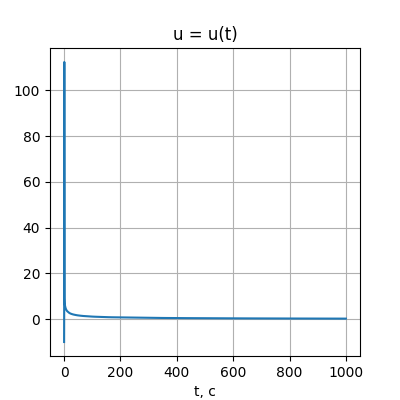
\includegraphics[width=0.65\textwidth]{1_u.png}
  \caption{График выхода регулятора неадаптивной системы управления.}
  \label{fig:task1_u}
\end{figure}

В этом задании параметр \(\theta\) системы принимается известным. 
Полученный результаты представлен на рис. \ref{fig:task1_y} - \ref{fig:task1_u}. 
Как видно, ошибка слежения является вычислительной погрешностью. 
Каждые 3 секунды происходит увеличение параметра \(\theta\) в 3 раза, что отражается на амплитуде выхода регулятора (рис.~\ref{fig:task1_u}).

\FloatBarrier
% \newpage
\subsection{Адаптивная система}
$$
    \begin{cases}
      \dot x_m = -\lambda x_m + \lambda g \\
      \dot x = \hat \theta x + u\\
      u = - \hat \theta x - \lambda x + \lambda g\\
      \varepsilon = x_m - x \\
      \dot{ \hat \theta} = -\gamma x \varepsilon 
    \end{cases} 
$$
\begin{figure}[h!]
    \centering
    \includegraphics[width=0.65\textwidth]{2_y.png}
    \caption{График ошибки слежения адаптивной системы управления.}
    \label{fig:task2_y}
\end{figure}
\begin{figure}[h!]
  \centering
  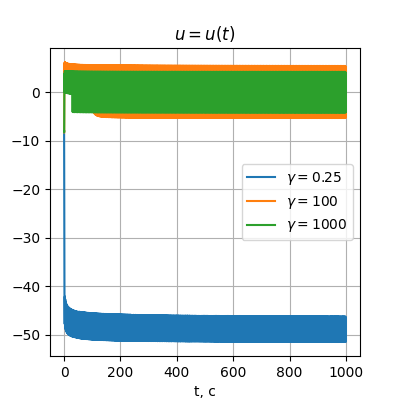
\includegraphics[width=0.65\textwidth]{2_u.png}
  \caption{График выхода регулятора адаптивной системы управления.}
  \label{fig:task2_u}
\end{figure}

\begin{figure}[h!]
  \centering
  \includegraphics[width=0.65\textwidth]{2_theta.png}
  \caption{График ошибки оценки параметра \( \theta\) адаптивной системы управления.}
  \label{fig:task2_theta}
\end{figure}

В этом задании параметр \(\theta\) неизвестен. 
Для управления используется алгоритм адаптации,
формирующий оценку \(\hat \theta\) при \(\gamma = 1000\). 
Полученный результат представлен на рис.~\ref{fig:task2_y}~-~\ref{fig:task2_theta}. 
Как видно, ошибка слежения \(\varepsilon\) и ошибка оценки неизвестного параметра \(\tilde {\theta}\) сходятся к 0.
\FloatBarrier
\subsection{Адаптивная система. Сравнение разных значений коэффициента адаптации}
\begin{figure}[h!]
  \centering
  \includegraphics[width=0.65\textwidth]{3_y.png}
  \caption{График ошибки слежения адаптивной системы управления при разных значениях коэффициента адаптации \(\gamma\).}
  \label{fig:task32_y}
\end{figure}
\begin{figure}[h!]
\centering
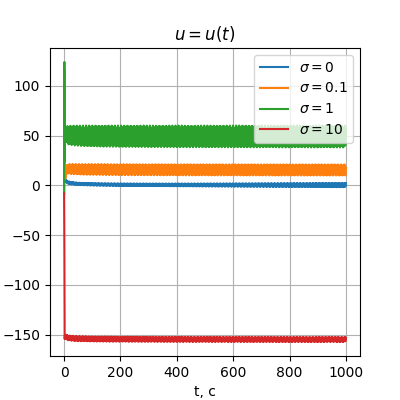
\includegraphics[width=0.65\textwidth]{3_u.png}
\caption{График выхода регулятора адаптивной системы управления при разных значениях коэффициента адаптации \(\gamma\).}
\label{fig:task32_u}
\end{figure}

\begin{figure}[h!]
\centering
\includegraphics[width=0.65\textwidth]{3_theta.png}
\caption{График ошибки оценки параметра \( \theta\) адаптивной системы управления при разных значениях коэффициента адаптации \(\gamma\).}
\label{fig:task32_theta}
\end{figure}
При разных значениях коэффициента адаптации (рис. \ref{fig:task32_y}~-~\ref{fig:task32_theta}) меняется скорость сходимости. Для больших коэффициентов процесс проходит быстрее, но и выход регулятора в начале больше.


\FloatBarrier
\newpage
\section{Заключение}
На практике подтвердилась работа адаптивного регулятора на примере задачи слежения выхода скалярного объекта за
эталонным сигналом.
Произведено сравнение влияния различных коэффициентов адаптации на сходимость. 



\bibliographystyle{unsrtnat}
\bibliography{ref}

\end{document}